\begin{figure}[H]
    \centering
    
\includegraphics[width=.95\linewidth]{img/Falessi/01_MetricheMisurazioni/nosb}
    \caption{}
    \label{fig:}
\end{figure}

\newpage
\chapter{Teoria della Misurazione e Scale di Misura}

\section{Introduzione alla Misurazione del Software}
La misurazione nel software engineering non è un fine, ma uno strumento decisionale di supporto. Come ricordano Lord Kelvin e Tom DeMarco, l'assenza di misurazione impedisce il controllo e, di conseguenza, il miglioramento dei processi e dei prodotti.

\subsection{Definizioni Formali}
Secondo i modelli standard, è necessario distinguere tre concetti fondamentali:
\begin{itemize}[label=\textbullet]
    \item \textbf{Misura (Measure):} Rappresentazione numerica di una caratteristica o di un attributo di un prodotto o processo software (es. 5000 LOC, 30 mesi-uomo).
    \item \textbf{Metrica (Metric):} La scala o il sistema di misurazione utilizzato per quantificare una misura. Definisce le regole di assegnazione dei valori (es. Complessità Ciclomatica, Densità dei Difetti).
    \item \textbf{Misurazione (Measurement):} Il processo pratico di assegnazione dei numeri alle misure utilizzando una metrica.
\end{itemize}

\subsection{Proprietà di una Metrica di Qualità}
Per essere considerata valida, una metrica deve soddisfare i seguenti criteri:
\begin{description}
    \item[Rilevanza:] Deve misurare un attributo significativo e importante del prodotto o processo software.
    \item[Oggettività:] Il risultato deve basarsi su dati verificabili e riproducibili, non su opinioni o stime soggettive.
    \item[Affidabilità e Consistenza:] La metrica deve produrre risultati costanti in condizioni diverse e deve essere coerente con gli obiettivi del progetto.
    \item[Usabilità:] Il calcolo e l'interpretazione devono essere facili, intuitivi e non richiedere sforzi o risorse eccessive.
\end{description}

\begin{notaprof}
La pertinenza di una metrica è strettamente legata al contesto di business. Un errore critico in un sistema assicurativo potrebbe riguardare l'accuratezza dei calcoli (oracolo) con conseguenze disastrose, mentre per un motore di ricerca come Google la priorità assoluta risiede nella disponibilità del servizio (uptime), dove anche poche ore di downtime globale risultano inaccettabili.
\end{notaprof}

\section{Tassonomia delle Scale di Misura}
La scelta della scala utilizzata dipende dalla natura dei dati misurati e determina quali operazioni statistiche siano matematicamente applicabili.

\subsection{Scala Nominale e Ordinale}
\begin{itemize}
    \item \textbf{Nominale:} Utilizzata per assegnare valori a etichette o categorie senza un ordine intrinseco o magnitudine (es. tipi di difetti: logica, UI, performance, sicurezza). Operazioni ammesse: Moda, frequenza.
    \item \textbf{Ordinale:} Prevede un ordine di rango per le categorie, ma la distanza o magnitudine tra i valori non è definita né significativa (es. priorità dei difetti: Critical, High, Medium, Low). Operazioni ammesse: Mediana.
\end{itemize}

\begin{notaprof}
Le scale ordinali, pur limitando le analisi statistiche alla mediana, offrono spesso una maggiore oggettività rispetto a scale numeriche forzate. Valutare la severità di un bug su una scala 0-100 introduce un'alta soggettività (es. la differenza tra 65 e 70 è arbitraria), mentre una distinzione qualitativa (Blocker vs Non-Blocker) risulta più robusta, netta e oggettiva.
\end{notaprof}

\subsection{Scale Numeriche (Intervallo e Rapporto)}
In queste scale i valori sono assegnati in ordine di rango e la magnitudine della differenza tra i punti ha un significato reale e misurabile.
\begin{itemize}
    \item \textbf{Intervallo:} La magnitudine delle differenze è significativa, ma non possiede uno zero assoluto reale.
    \item \textbf{Rapporto (Ratio):} È il tipo di scala più sofisticato, in cui la magnitudine delle differenze è calcolabile e possiede uno zero assoluto reale (es. LOC, sforzo, tempo).
\end{itemize}
\textbf{Statistiche ammesse per entrambe:} Media, Deviazione Standard, Varianza, Range. Per la scala di Rapporto sono ammessi anche coefficiente di variazione e media geometrica.


\begin{figure}[H]
    \centering
    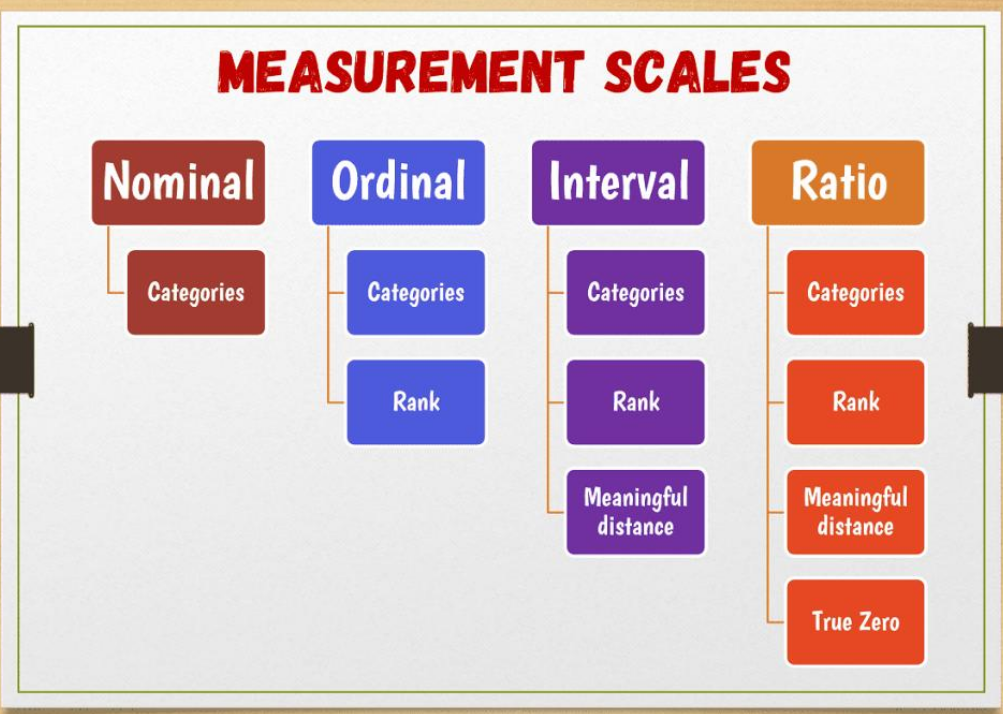
\includegraphics[width=.65\textwidth]{img/Falessi/01_MetricheMisurazioni/mm}
    \caption{Scale di Misura: Nominale, Ordinale, Intervallo e Rapporto.}
    \label{fig:mm}
\end{figure}


\section{Modelli di Qualità: Lo Standard ISO/IEC 25010}
Lo standard ISO 25010 definisce una tassonomia dettagliata degli attributi di qualità, distinguendo tra qualità del prodotto e qualità in uso. Le caratteristiche principali individuate dallo standard sono:
\begin{enumerate}
    \item \textbf{Functional Suitability (Adeguatezza funzionale):} Completezza, correttezza e adeguatezza funzionale.
    \item \textbf{Performance Efficiency (Efficienza delle prestazioni):} Comportamento temporale, utilizzo delle risorse e capacità strutturale.
    \item \textbf{Security (Sicurezza):} Riservatezza, integrità, non ripudio, responsabilità e autenticità.
    \item \textbf{Maintainability (Manutenibilità):} Modularità, riusabilità, analizzabilità, modificabilità e testabilità.
\end{enumerate}

\begin{notaprof}
È cruciale distinguere sempre il modello di qualità dalle metriche: il modello, come l'ISO 25010, definisce \textit{cosa} significa la qualità fornendone una tassonomia, mentre le metriche definiscono \textit{come} quantificarla operativamente. L'adozione di questi standard fallisce sistematicamente se manca la ``buona fede'' aziendale; l'uso delle metriche al solo scopo di ottenere certificazioni formali di facciata, senza mirare a un miglioramento sostanziale del prodotto, svilisce l'utilità dell'intero sistema di valutazione ingegneristico.
\end{notaprof}

\section{Introduzione alle Metriche Object-Oriented}
Le metriche object-oriented vengono impiegate per misurare la qualità dei sistemi software ad oggetti e identificare tempestivamente difetti di progettazione o futuri problemi di manutenibilità. Vanno sempre interpretate come indicatori di rischio e valutate in modo comparativo, rispetto a una baseline o a un trend, e non in senso assoluto.

\begin{notaprof}
In ambito manageriale, è molto più efficace adottare un approccio pratico basato sulle distribuzioni piuttosto che sulle medie globali. Risulta strategicamente più utile concentrare le attività di analisi, refactoring e test mirati esclusivamente sul 10\% delle classi che presentano i valori peggiori di complessità (\textit{outliers}), piuttosto che tentare di ottimizzare e riscrivere l'intero sistema in modo uniforme.
\end{notaprof}

\chapter{Software Metrics and Their Use}

\section{Metriche software e decisioni}

Le \textbf{metriche software} sono strumenti di supporto alle decisioni ingegneristiche. Non rappresentano una verità assoluta sul sistema e non devono essere interpretate come giudizi automatici sulla qualità.

\begin{notaesame}
Una metrica ha senso solo se è collegata a un obiettivo, a un contesto e a una decisione concreta. Un valore alto o basso non è automaticamente positivo o negativo.
\end{notaesame}

Il processo di misurazione può essere visto come una \textbf{measurement-to-decision pipeline}:

\begin{enumerate}
    \item \textbf{Goal / Decision}: quale decisione si vuole supportare?
    \item \textbf{Operational definition}: cosa si misura, su quale artefatto e con quali regole?
    \item \textbf{Collection}: raccolta dei dati tramite strumenti e procedure definite.
    \item \textbf{Analysis}: analisi tramite baseline, trend, distribuzioni o test statistici.
    \item \textbf{Interpretation rule}: regole per interpretare i valori osservati.
    \item \textbf{Action}: azione conseguente, come refactoring, redesign o modifica della strategia di test.
\end{enumerate}

\begin{notaprof}
Raccogliere dati senza sapere quale decisione prendere è inutile. Una metrica non ha valore perché produce un numero, ma perché aiuta a decidere cosa fare.
\end{notaprof}

Anche la scala di misura è importante. Una scala ordinale, come \emph{low}, \emph{medium}, \emph{high}, può essere più robusta per descrivere concetti qualitativi, ma limita le operazioni statistiche. Una scala numerica permette calcoli come media e varianza, ma può introdurre soggettività se i numeri non hanno un significato operativo chiaro.

\section{Quality model vs metrics}

È fondamentale distinguere tra \textbf{modello di qualità} e \textbf{metrica}.

\begin{itemize}
    \item Il \textbf{modello di qualità} definisce \emph{cosa} significa qualità in un certo contesto.
    \item La \textbf{metrica} definisce \emph{come} quantificare operativamente uno specifico attributo.
\end{itemize}

Per esempio, un modello di qualità può stabilire che la manutenibilità è rilevante; una metrica può poi provare a quantificarla tramite complessità, accoppiamento, coesione o code smells.

\begin{notaprof}
Applicare metriche e standard senza un reale obiettivo di business rende la misurazione sterile. Se un'organizzazione usa le metriche solo per rispettare formalmente un contratto, senza voler migliorare davvero il prodotto, il processo perde significato ingegneristico.
\end{notaprof}

\begin{notaesame}
Non bisogna scegliere una metrica prima di sapere quale decisione deve supportare. Una metrica senza contesto decisionale è solo un numero.
\end{notaesame}

\section{ISO/IEC 25010}

Lo standard \textbf{ISO/IEC 25010} fornisce una tassonomia degli attributi di qualità del software. Serve a costruire un vocabolario condiviso per descrivere qualità del prodotto e qualità in uso.

\begin{notaslide}
ISO/IEC 25010 può essere usato per specificare requisiti, pianificare attività di Quality Assurance, definire criteri di accettazione e supportare attività di benchmarking.
\end{notaslide}

Lo standard indica quali dimensioni della qualità considerare, ma non definisce automaticamente quali metriche usare, quali soglie applicare o quali decisioni prendere.

Le caratteristiche principali richiamate sono:

\begin{itemize}
    \item \textbf{Functional suitability}: completezza, correttezza e appropriatezza funzionale;
    \item \textbf{Performance efficiency}: comportamento temporale, uso delle risorse e capacità;
    \item \textbf{Security}: confidenzialità, integrità e non ripudio;
    \item \textbf{Maintainability}: modularità, riusabilità, analizzabilità e testabilità.
\end{itemize}

\begin{notaesame}
ISO/IEC 25010 aiuta a definire cosa osservare nella qualità del software, ma non sostituisce la scelta delle metriche né l'interpretazione ingegneristica dei risultati.
\end{notaesame}

\section{Metriche Object-Oriented}

Le \textbf{metriche Object-Oriented} servono a individuare possibili problemi di progettazione, manutenibilità, testing e comprensione del codice nei sistemi a oggetti.

\begin{notaesame}
Le metriche OO devono essere lette come \textbf{indicatori di rischio}. Un valore critico non dimostra automaticamente che una classe sia sbagliata, ma segnala che quella classe merita attenzione.
\end{notaesame}

L'interpretazione deve essere comparativa e contestuale. È utile osservare baseline di progetto, trend nel tempo, distribuzioni, outlier e confronto tra classi simili.

\begin{notaprof}
Non ha senso cercare una soglia universale valida per tutte le classi. È più utile osservare il peggior 10\% delle classi del progetto e concentrarsi sugli outlier.
\end{notaprof}

\section{CK Metrics}

\begin{notaslide}
La suite CK, proposta da Chidamber e Kemerer, valuta aspetti come complessità, ereditarietà, accoppiamento e coesione nei sistemi object-oriented.
\end{notaslide}

\begin{description}
    \item[WMC -- Weighted Methods per Class:] misura la complessità complessiva dei metodi di una classe, spesso approssimata tramite il numero di metodi. Un valore alto può indicare troppe responsabilità, maggiore difficoltà di testing e possibile necessità di dividere la classe.

    \item[DIT -- Depth of Inheritance Tree:] misura la profondità della classe nella gerarchia di ereditarietà. Un valore alto può indicare riuso, ma anche maggiore difficoltà di comprensione e rischio di interazioni inattese tra classi base e derivate.

    \item[NOC -- Number of Children:] misura il numero di sottoclassi immediate. Un valore alto indica che la classe base è molto riutilizzata, ma anche che una sua modifica può generare regressioni in molte sottoclassi.

    \item[CBO -- Coupling Between Object Classes:] misura quante classi distinte sono accoppiate a una classe. Un valore alto indica rischio di bassa modularità, \emph{ripple effects} e difficoltà di testing isolato.

    \item[RFC -- Response For a Class:] misura il numero di metodi che possono essere eseguiti in risposta a un messaggio ricevuto dalla classe. Un valore alto indica comportamento complesso e ampia superficie di test.

    \item[LCOM -- Lack of Cohesion in Methods:] misura la mancanza di coesione tra i metodi. Un valore alto può indicare che la classe contiene responsabilità diverse fuse insieme, suggerendo un possibile refactoring.
\end{description}

\begin{notaesame}
Le CK metrics non dicono automaticamente che una classe è errata. Servono a individuare classi potenzialmente rischiose da analizzare con attenzione.
\end{notaesame}

\section{Altre metriche}

La \textbf{Cyclomatic Complexity} misura la complessità del flusso di controllo di un metodo o programma. Cresce in presenza di strutture decisionali come \texttt{if}, \texttt{while}, \texttt{for} e \texttt{switch}.

\begin{notaslide}
Nel testing, la Cyclomatic Complexity può essere usata per stimare il numero minimo di casi necessari a coprire i percorsi di base.
\end{notaslide}

Un valore alto indica spesso codice più difficile da comprendere, mantenere e testare. Tuttavia, non bisogna interpretare il valore in modo meccanico: alcuni problemi sono intrinsecamente complessi.

Il \textbf{Fan-in} misura quante classi o componenti dipendono da una certa classe. Se è alto, la classe è critica perché molto usata. Il \textbf{Fan-out} misura invece da quante classi o componenti dipende una classe; se è alto, può indicare forte dipendenza dal resto del sistema.

\begin{notaprof}
Non bisogna rifattorizzare tutto automaticamente. Una classe può essere complessa o molto connessa perché il problema che risolve è intrinsecamente complesso. Separare artificialmente responsabilità non divisibili può peggiorare la manutenibilità.
\end{notaprof}

Le metriche possono essere osservate a diversi livelli:

\begin{itemize}
    \item \textbf{method-level}: Cyclomatic Complexity, nesting depth;
    \item \textbf{class-level}: LOC, WMC, CBO, RFC, LCOM;
    \item \textbf{package/module-level}: accoppiamento afferente, accoppiamento efferente, instability;
    \item \textbf{process-level}: code churn, frequenza di modifica, ownership concentration.
\end{itemize}

Le metriche di processo sono spesso molto predittive perché descrivono come il codice evolve nel tempo, non solo come appare in uno snapshot.

\section{Function Points}

I \textbf{Function Points} sono una metrica usata per stimare la grandezza funzionale di un sistema software. Sono indipendenti dal linguaggio di programmazione, dalla tecnologia, dal framework e dall'implementazione concreta.

\begin{notaesame}
I Function Points sono un argomento frequente nelle domande d'esame.
\end{notaesame}

L'idea centrale è misurare il software dal punto di vista dell'utente o del business. Per questo motivo sono utili nelle fasi iniziali del progetto, quando il codice non esiste ancora ma sono già disponibili requisiti o descrizioni funzionali.

Un concetto fondamentale è l'\textbf{application boundary}, cioè il confine tra ciò che appartiene all'applicazione e ciò che è esterno.

\begin{notaslide}
L'application boundary stabilisce cosa è interno al sistema e cosa deve essere considerato esterno.
\end{notaslide}

Il calcolo dei Function Points si basa su cinque categorie:

\begin{itemize}
    \item \textbf{ILF (Internal Logical File)}: dati mantenuti internamente dall'applicazione;
    \item \textbf{EIF (External Interface File)}: dati usati dall'applicazione ma mantenuti esternamente;
    \item \textbf{EI (External Input)}: transazioni in ingresso che modificano dati interni;
    \item \textbf{EO (External Output)}: transazioni in uscita che producono informazioni derivate;
    \item \textbf{EQ (External Inquiry)}: interrogazioni che leggono dati senza modificarli.
\end{itemize}

I Function Points possono essere usati per stimare dimensione funzionale, effort, costi, schedule e produttività attesa. Per ottenere stime realistiche, è necessario calibrare i valori usando dati storici dell'organizzazione.

\subsection{Vantaggi e svantaggi dei Function Points}

I \textbf{Function Points} hanno diversi vantaggi. Il principale è che permettono di stimare la dimensione funzionale del sistema prima che il codice venga scritto. Questo li rende utili nelle fasi iniziali del progetto, quando sono disponibili requisiti e descrizioni funzionali, ma non ancora l'implementazione.

Un altro vantaggio è la loro indipendenza dalla tecnologia. Poiché non dipendono dal linguaggio di programmazione, dal framework o dall'architettura scelta, consentono di confrontare sistemi sviluppati con tecnologie diverse. Inoltre, essendo basati sul punto di vista dell'utente o del business, aiutano a collegare la stima tecnica alle funzionalità realmente percepite dagli stakeholder.

\begin{notaslide}
I Function Points sono particolarmente utili per stime preliminari di size, effort, costi e schedule, soprattutto quando vengono calibrati con dati storici di produttività dell'organizzazione.
\end{notaslide}

Tuttavia, i Function Points presentano anche alcuni limiti. Il calcolo richiede interpretazione e può quindi introdurre soggettività, soprattutto nella definizione dell'application boundary e nella classificazione di ILF, EIF, EI, EO ed EQ. Due analisti diversi potrebbero produrre stime differenti se non condividono criteri operativi chiari.

Inoltre, i Function Points misurano la dimensione funzionale, ma non catturano direttamente aspetti non funzionali come performance, sicurezza, affidabilità, usabilità o complessità tecnica. Per questo motivo, due sistemi con gli stessi Function Points possono richiedere effort molto diversi se uno dei due ha requisiti extra-funzionali più stringenti.

\begin{notaesame}
Il vantaggio dei Function Points è che permettono una stima precoce e indipendente dalla tecnologia. Il limite principale è che non misurano direttamente qualità, complessità tecnica o requisiti non funzionali.
\end{notaesame}

\begin{notaprof}
I Function Points ignorano molti requisiti non funzionali. Due sistemi con le stesse funzionalità possono avere lo stesso numero di Function Points, anche se uno deve essere molto più sicuro, performante o robusto.
\end{notaprof}

\begin{notaesame}
I Function Points non misurano direttamente la qualità. Misurano la dimensione funzionale del sistema dal punto di vista utente/business.
\end{notaesame}

\section{GQM+Strategies}

\textbf{GQM+Strategies} estende l'approccio Goal-Question-Metric collegando obiettivi di business, obiettivi software, domande, misure, strategie e target.

\[
\text{Business Goals}
\rightarrow
\text{Software Goals}
\rightarrow
\text{Questions}
\rightarrow
\text{Measures}
\rightarrow
\text{Strategies / Targets}
\]

L'idea è che ogni metrica debba rispondere a una domanda, ogni domanda debba essere collegata a un obiettivo e ogni obiettivo debba avere senso rispetto alla strategia dell'organizzazione.

\begin{notaprof}
Tutto nasce dalla modellazione del business. Se non si definisce come l'organizzazione ottiene successo, qualsiasi metrica o attività di refactoring può diventare inutile o persino dannosa.
\end{notaprof}

Per esempio, l'obiettivo generico ``migliorare la qualità'' può essere trasformato in una domanda come ``la copertura dei test è sufficiente?'', associato a una misura come la code coverage e collegato a una strategia come aumentare la copertura introducendo nuovi unit test.

\begin{notaslide}
Il reference process di GQM+Strategies include le fasi Initialize, Characterize, Set Goals, Choose Process, Execute Model, Analyze Results, Package and Improve.
\end{notaslide}

\begin{description}
    \item[Initialize:] avvio dell'attività di misurazione.
    \item[Characterize:] analisi del contesto organizzativo e progettuale.
    \item[Set Goals:] definizione degli obiettivi.
    \item[Choose Process:] scelta del processo di misurazione.
    \item[Execute Model:] esecuzione del modello.
    \item[Analyze Results:] analisi dei risultati.
    \item[Package and Improve:] consolidamento della conoscenza e miglioramento futuro.
\end{description}

\begin{notaesame}
GQM+Strategies serve ad allineare le metriche alle decisioni organizzative. Una metrica è utile solo se risponde a una domanda collegata a un obiettivo.
\end{notaesame}

\section{Collegamento con il progetto}

Nel progetto, le metriche vengono usate per analizzare il software, costruire dataset, stimare la difettosità e valutare il refactoring. Non basta calcolare valori numerici: bisogna interpretarli e collegarli a decisioni concrete.

\begin{notaesame}
Nel progetto le metriche devono supportare decisioni come individuare classi rischiose, valutare bugginess, scegliere dove intervenire, analizzare l'effetto del refactoring e discutere i risultati.
\end{notaesame}

Le metriche possono essere estratte a livello di classe, per esempio tramite SonarCloud, e possono contribuire alla costruzione del dataset di defect prediction. Possono inoltre aiutare a identificare classi più rischiose, confrontare versioni prima e dopo un refactoring e discutere il rapporto tra maintainability, testing e code smells.

Nel caso del refactoring automatico tramite LLM, l'analisi deve verificare se la nuova versione della classe:

\begin{itemize}
    \item compila correttamente;
    \item preserva la funzionalità originale;
    \item supera i test;
    \item riduce i code smells;
    \item non peggiora metriche correlate positivamente con la bugginess.
\end{itemize}

\begin{notaprof}
Il valore del progetto non dipende dal fatto che l'LLM produca sempre un refactoring perfetto, ma dalla capacità di interpretare i risultati e prendere decisioni motivate sulla base dei dati raccolti.
\end{notaprof}

Gli errori comuni da evitare sono:

\begin{itemize}
    \item usare medie globali senza analizzare distribuzioni e outlier;
    \item applicare soglie arbitrarie come se fossero verità assolute;
    \item presentare metriche senza spiegare quale decisione supportano;
    \item ignorare la complessità intrinseca del problema;
    \item interpretare ogni valore alto come necessariamente negativo;
    \item non spiegare il razionale dietro le scelte di misurazione.
\end{itemize}

\begin{notaesame}
Una buona discussione progettuale non si limita a mostrare numeri. Deve spiegare cosa significano quei numeri, quali decisioni supportano e quali limiti hanno.
\end{notaesame}